\documentclass[a4paper, 10.5pt,twocolumn,dvipdfmx]{jsarticle}

%\usepackage[a4paper,top=10truemm,bottom=10truemm,left=1truemm,right=1truemm]{geometry}
\usepackage{amsmath}
\usepackage{amsfonts}
\usepackage{eshouroku}
\usepackage[dvipdfmx]{graphicx}
\usepackage{amsmath}
\usepackage{url}
\usepackage{here}
\usepackage{booktabs}
\usepackage{remreset}
\usepackage{pdfpages}
\usepackage{comment}
\usepackage{subfigure}
\usepackage{amsmath}
\usepackage{titlesec}
\pagestyle{empty}
\setlength{\columnsep}{2zw}
\newcommand{\ctext}[1]{\raise0.2ex\hbox{\textcircled{\scriptsize{#1}}}}

\titleformat*{\section}{\normalsize\bfseries}
\titleformat*{\subsection}{\small\bfseries}
\titleformat*{\subsubsection}{\small\bfseries}
\renewcommand{\baselinestretch}{0.9}

\renewcommand{\subfigtopskip}{1pt}	% 図の上の隙間。上図の副題と下図の間。
\renewcommand{\subfigbottomskip}{0pt} % 図の下の隙間。副題と本題の間。
\renewcommand{\subfigcapskip}{-6pt}	% 図と副題の間
\renewcommand{\subcapsize}{\scriptsize} % 副題の文字の大きさ

\makeatletter
	\renewcommand{\theequation}{% 式番号の付け方
	\thesection\arabic{equation}}
	\@addtoreset{equation}{section}

	\renewcommand{\thefigure}{% 図番号の付け方
	\thesection\arabic{figure}}
	\@addtoreset{figure}{section}

	\renewcommand{\thetable}{% 表番号の付け方
	\thesection\arabic{table}}
	\@addtoreset{table}{section}
\makeatother
%\numberwithin{equation}{section}
%\numberwithin{table}{section}
%\numberwithin{figure}{section}


% 数式(演算子など)のスペースを詰める
% =,→ 間の余白
\thickmuskip=1.0\thickmuskip
% +,- 間の余白
\medmuskip=0.8\medmuskip
% … などの装飾記号の余白
\thinmuskip=0.8\thinmuskip
% 行列を詰める
\arraycolsep=0.3\arraycolsep
% 数式の上下のスペースの変更
\AtBeginDocument{
  \abovedisplayskip     =0.5\abovedisplayskip
  \abovedisplayshortskip=0.5\abovedisplayshortskip
  \belowdisplayskip     =0.5\belowdisplayskip
  \belowdisplayshortskip=0.5\belowdisplayshortskip}


%\boldmainfalse% 主文を普通文字にするモード(抄録印刷時はこちら)
\graphicspath{{./figs}}

\begin{document}

\twocolumn[
 \講演番号{B-11}% 必要ない場合には書かない
 \日本語タイトル{\huge}{神経免疫相互作用に着想を得た\\マルチエージェントシステム型ニューラルネットワークの提案}
 \英語タイトル{\large}{Proposal of Neural Network composed of Multi-Agent System Inspired by Neuroimmune Interaction}
 \筆者一名{5335}{柚木開登}

 \指導教員一名{山本哲也}
 %\指導教員二名{東京花子}{京都紀夫}
 %\指導教員なし
]
%\addcontentsline{toc}{section}{\refname}% 追加

\graphicspath{{./figs/}} % 図が特定のフォルダにある場合には設定

\section{本研究の意義・目的}
\begin{comment}
本来的に大規模な計算資源を必要とするニューラルネットワークが
今日, あらゆる産業へ導入されるに至ったのは, クラウドコンピューティングの貢献がある.
一方で, 同市場拡大に伴って
プラットフォーマによる市場寡占, データセンターでの電力消費, データプライバシーの課題が表面化した.
こうしたクラウドの課題克服に向けて, 
データを集約せずにネットワークの端点(エッジ)で処理するエッジコンピューティングが注目
されている.
\end{comment}
大規模なニューラルネットワークの学習には, 本来的に豊富な計算資源を必要とするが, 
今日では, クラウドコンピューティングの発展によって, 
低いコストで大規模なモデルの構築・学習が可能となっており, その結果として
多様な製品開発・サービスに機械学習の導入が広まっている.

一方で, このようなクラウド依存な機械学習は, 
その性質上, 他の製品開発に流用可能性がある大量の学習データを集約するため, 
悪意の第三者, あるいはプラットフォーム企業そのものによって盗取される可能性が否定できない.
特に近年では「個人に最適化された情報」への需要から, 
学習データに顔写真・年齢・性別・信条・趣味嗜好を含めたあらゆる個人情報が
含まれることが多く, その流出リスクは大きい.

さらに, 2013年のアメリカ国家安全保障局(NSA)による大量監視プログラム発覚以降, 
EUの一般データ保護規則をはじめとして世界各国が巨大IT企業を意識した個人情報保護に係る規制を強めており, 
機械学習における個人情報の扱いは変革が迫られている.

上述した課題を解決すると期待されるのが, 連合学習(Federareted Learning; FL)\cite{DFL}である. 
連合学習では, 学習データを集約するのではなく, 
ローカルな学習データを保有する各ノードが, 個々に学習を行い,
その結果得たパラメータ差分を他のノードと通信し平均化することで大規模な
学習済みモデルを構築する. 
これによって, プライバシーを含んだ学習データは通信されず個人情報がノード内に保護される.

連合学習の実用化に際しては, 従来データセンターで学習されていた大規模なニューラルネットワークを
計算資源に乏しい利用者側の計算機環境(エッジ環境)に投入する必要があるため,  
「モデルの軽量化」及び「環境内計算資源の有効利用」の両方面のアプローチが重要である.
前者に対しては, 不要なシナプスを除去するPruning(剪定, 刈り込み), 
後者に対しては複数の不均一計算資源への
ニューラルネットワークの分散化といったアイデアが提案されているものの, 
両アプローチを兼ね備えたモデルは提案されてこなかった.

そこで本研究では, モデルの軽量化および分散化を兼ね備えたモデルを構成することを目的に, 
神経免疫相互作用を考慮した複数の自律行動主体(エージェント)で構成されるニューラルネットワークを検討を行う.
\section{提案モデル}
\subsection{複数のエージェントで構成されるニューラルネットワーク}
本提案はモデルを構成する個々のユニットを自律行動主体(エージェント)として解釈しており, 
具体的には, 情報の変換を行うNeuro-Agent, Neuro-Agent間の情報の伝達を担うSynapse-Agent, 
それらによって構成されるニューラルネットワークに対して不要なシナプスの刈り込みを行うGlia-Agent
によって構成されている.以下, それぞれについて説明する.
\vspace{2mm}
  \subsubsection*{● Neuro-Agent;\,\,NA}
  神経細胞をモデル化したエージェントであり, 情報の受容, 処理, 
  転送などを担当する.
  それぞれのNeuro-Agent(以降, NA)は, 情報を受け取るための複数の入力$x_i$ $\;(i= 1, 2, 3, \cdots m)$と, 
  バイアス$b$を持ち, 
  これを処理して別のNAに情報を送信するための出力$y$を生成する.
  この時の内部処理は\weq{Neuro-Agent}に示す通り, 
  標準的な人工ニューロンと同等に活性化関数$\phi$を用いた変換である.
  \begin{align}
    y=\phi(\sum_{i=1}^m x_i+b)
    \label{eq:Neuro-Agent}
  \end{align}
  \subsubsection*{●Synapse-Agent;\,\,SA}
  神経回路における接触構造であるシナプスをモデル化したエージェントであり, 
  NA間の情報の伝達を担当する.
  それぞれのSynapse-Agent(以降SA)は, NAからの出力$y$を受け取り, それを変換した値$x$を出力する(\weq{Synapse-Agent}). 
  この出力は別のNAの入力として使用される.
  \begin{align}
    x=w\cdot y
 \label{eq:Synapse-Agent}   
  \end{align}
  ここで, 式中の$w$は, そのSAの重みを示し, 
  これとNAのバイアス$b$について出力の誤差に対する責任を計算することで学習を行う(誤差逆伝播法).
  \vspace{2mm}
  \subsubsection*{●Glia-Agent;\,\,GA}
  神経細胞の補助細胞であるグリア細胞の機能を模倣したエージェント. 
  Glia-Agent(以降GA)は, NAと1:1で接続され, この接続を介して, 
  NAとSAで構成されるニューラルネットワーク中の不要なシナプスの刈り込みを試みる.
  \vspace{2mm}
\subsection{神経免疫相互作用に基づく相互調節モデル}
グリア細胞の一種で脳内免疫細胞であるmicrogliaは, 抗原提示や貪食といった役割のほかに,  
シナプス形成における神経回路の刈り込みの実行者という側面を持つ. 
このようなmicrogliaの作用に対し, 
神経細胞はcytokine, chemokine, 核酸などのシグナル伝達物質を産生することで, 
能動的にmicrogliaを制御することが知られている. 
本モデルではこの脳内における細胞間の神経免疫相互作用(Neuroimmune Interaction)を
模倣し,
\wfig{NeuroGlia}に示すNAとGAの相互作用として組み込んだものである.
\vspace{-1.5zh}
\begin{figure}[H]
  \centering
  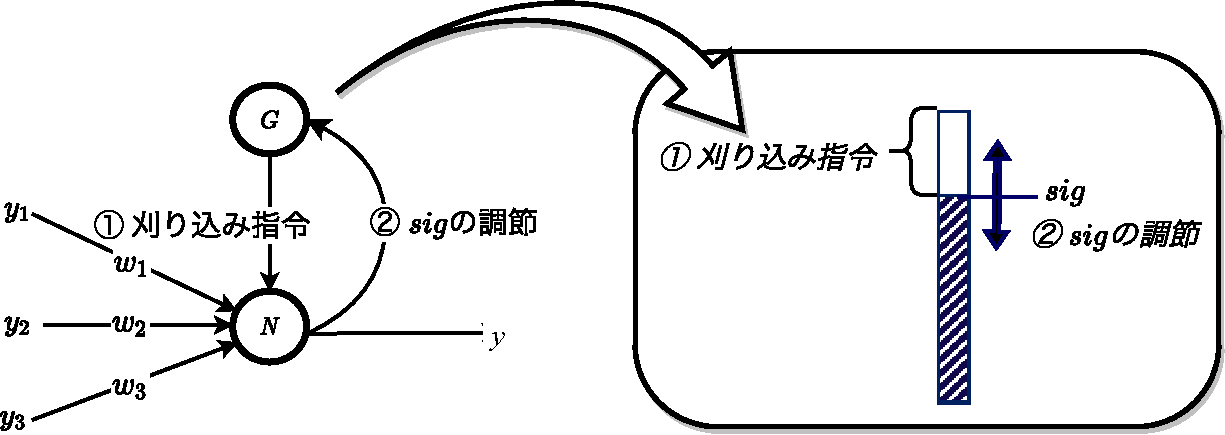
\includegraphics[width=10cm]{NewDeal-crop.pdf}
  \caption{Neuro-Glia相互調節機構}
  \label{fig:NeuroGlia}
\end{figure}
\vspace{-2zh}
\vspace{2mm}
\subsubsection{GAからNAへの作用\,\,:\,\,刈り込み命令}
シナプスの刈り込み命令はGAの内部変数$sig$
を閾値に用いて確率的に実行される.
NAは刈り込み命令を受け取ると, 自身に接続された最も重みが0に近いSAを
削除する.
また, 刈り込み指令を発出したGAは
$sig=1.0$に更新し, グリアネットワークへの伝播を行う.
詳しくは2.3節で述べるが, これに拠って時空間的に集中した過度な刈り込みが抑制される.

\vspace{2mm}
\subsubsection{NAからGAへの作用\,\,:\,\,$sig$の更新}
NAはまず, データ数$miniBatchSize$の間に
隣接するNAの出力値と比較し, 自分が外れ値であった回数を変数$cnt$にカウントする.
次に, $cnt$を用いて自身の活動頻度$f$を計算する.
\begin{align}
  f=\displaystyle\frac{cnt}{miniBatchSize}
\end{align}
最後に$f$を用いて, GAの内部変数$sig$を更新する.
$sig$の更新式は\weq{sig}に示す通りである. 
ただし, わかりやすさのため式中でGlia-Agentのプロパティには$G$, 及び
NAのプロパティには$N$の添字を付してある.
\begin{align}
  sig_G\leftarrow sig_G-&\alpha\left[\cfrac{2}{1-\beta\exp(freq_N-0.01)}-1\right]
  \label{eq:sig}
\end{align}
\weq{sig}は, NAの活動頻度$f$が高いほど刈り込みを抑制し, 逆に$f$が小さいほど
刈り込みがされやすくなるように$sig$を更新する.
\subsection{グリアネットワークによる過度な刈り込みの抑制}
神経免疫疾患の
グリア細胞は相互に, 情報伝達を行なっている.このグリア同士のネットワークは, 
グリアアセンブリ(Glia-Assembly)と呼ばれ, 数々の動物実験から
シナプス形成や脳機能維持に重要な役割を果たしていることが示唆されている. 

本提案では, グリアアセンブリを模倣したGA同士のネットワークであるグリアネットワークを導入する.
GAは刈り込み指令を下した際に, $sig=1.0$に更新し, 周囲の
GAに自身の$sig$の影響を伝播させる. 
グリアネットワーク上において$sig$は伝播距離(ホップ数)に応じて減衰率$A$だけ減衰していく.
なお, 複数の距離が与えられた場合, 最も近いGAの影響を優先する.
例えば, \wfig{GliaNetworks}の$G_1$の場合, 
$G_1\rightarrow G_2\rightarrow G_3\rightarrow G_4$と$G_k\rightarrow G_4$の経路では後者の経路のみを考えることになる.
\vspace{-1.5zh}
\begin{figure}[H]
  \centering
  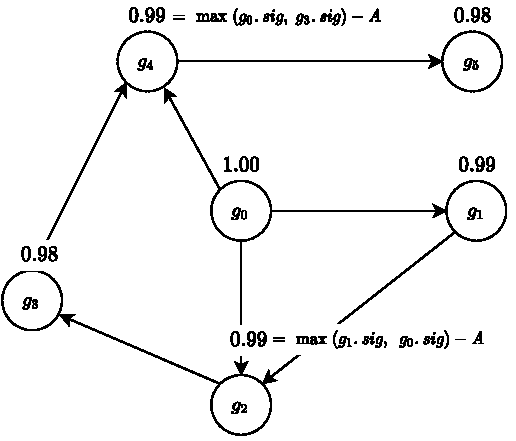
\includegraphics[width=8cm]{GliaNetworks.pdf}
  \caption{グリアネットワークでの$sig$の伝播のあり方}
  \label{fig:GliaNetworks}
\end{figure}
\vspace{-2zh}
一般に, $G_i \,,\,(i\in 1,2,3\cdots m)$からの入力をもつグリア$G$の$sig$の更新値は
以下のようになる.
\begin{align}
  sig_{G}=\min(sig_{G_i})-A
\end{align}
\section{計算機実験}
計算機実験として$6\rightarrow 8\rightarrow 8\rightarrow 8\rightarrow 1$の
5層全結合ニューラルネットワークを用意し, 
6bitの入力の上位3bitのいずれかに1が入っているかどうか
の判別のタスクを行った.
その他のパラメータは以下に示す通りである(\wtab{param}).
\vspace{-0.5cm}
\begin{table}[H]
  \caption{パラメータ一覧}
  \label{tab:param}
  \centering
  \scalebox{0.9}{
   \begin{tabular}{ll}
    \toprule
      パラメータ&値\\\midrule\midrule
      学習率$\eta$&$0.5$\\
      ミニバッチサイズ$miniBatchSize$&$100$\\
      初期抑制信号値$sig$&0.5\\
      減衰率$A$&0.01\\
      チューニングパラメータ$\alpha$&0.01\\
      チューニングパラメータ$\beta$&$6\ln(3)$\\
    \bottomrule
   \end{tabular}
  }
 \end{table}
計算機実験の結果得られた学習曲線及びシナプス数の変化及び, 刈り込み後のネットワークを
\wfig{SynapseNum}及び\wfig{Graph}に示す.
\begin{figure}[H]
  \centering
  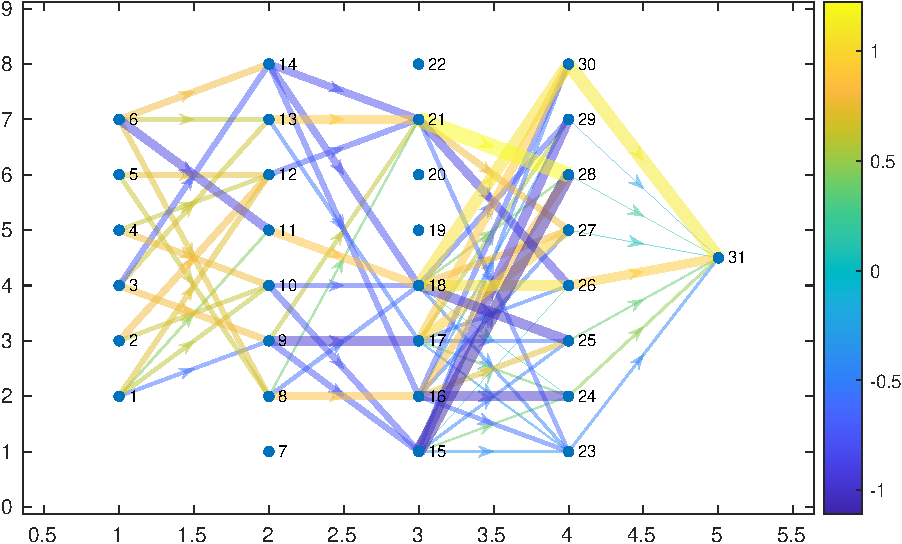
\includegraphics[width=8cm]{Graph-crop.pdf} 
  \caption{学習曲線}
  \label{fig:Graph}
\end{figure}
\vspace{-2zh}
\begin{figure}[H]
  \centering
  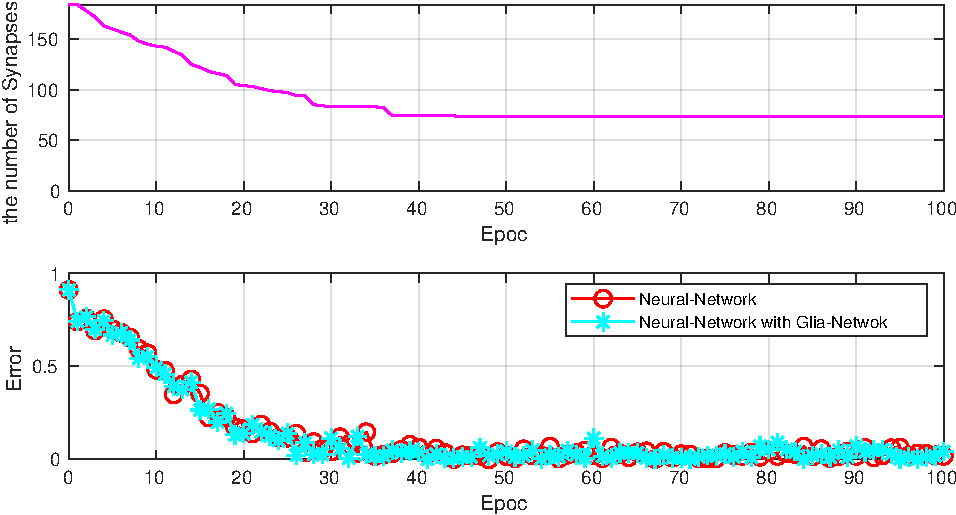
\includegraphics[width=8cm]{Subploting-crop.pdf} 
  \caption{シナプス量の変化(上図)と学習曲線(下図)}
  \label{fig:SynapseNum}
\end{figure}
\vspace{-2zh}

学習誤差率の時間変化を\wfig{SynapseNum}上図に示す。赤丸は刈り込みを行った場合、青丸が刈り込みを行わない場合の結果である。結果からわかるように、刈り込みによる学習率の低下は見られなかった。また、ニューラルネットワークのシナプス数の時間変化を図3.1下図に示す。結果からわかるように約40エポックまでにシナプスが刈り込まれ減少し、その後一定数に収束していることがわかる。これらのシナプス数の減少は指数関数的であり、オーバーシュート型シナプス形成の同様の傾向を示していた。
具体的には、初期の結合のシナプス数182が、最終的に72まで減少し、約60のシナプスが削減された。実際の刈り込み後のネットワークを\wfig{Graph}に示す.
赤が正の結合、青が負の結合を表、絶対値が大きいほど太い線で表ている.
最終結果のネットワークでは、入力層、出力層のニューロン全ての結合は維持されており、中間層において主に刈り込みが生じていることが確認できた。
以上のことから、提案システムにより、学習精度を維持したままモデルの削減が行えることが確認できた。
\section{結論}
GAの刈り込み発出確率は、NAの活動量および近隣のGAの刈込み発出により変動するようにした.
その結果、学習率の精度を低下させることなく約60%のシナプスの削減できることを確認した.
今後の課題は、刈込み過ぎによる学習精度の劣化を軽減するための方策(人での知見を参考にした刈り込みタイミング)の検討が考えられる。
 \begin{thebibliography}{99}
  \bibitem{DFL} 	
  Roy, Abhijit Guha, et al. "Braintorrent: A peer-to-peer environment for decentralized federated learning." arXiv preprint arXiv:1905.06731 (2019).
\end{thebibliography}
 \end{document}
